\documentclass{llncs}

\usepackage{cite}
\usepackage[pdftex]{graphicx}
\usepackage{url}
\usepackage{placeins}

\newif\iflong
\longfalse

% correct bad hyphenation here
\hyphenation{op-tical net-works semi-conduc-tor}


\begin{document}
%
\title{Federated Identity and Access Management for the Internet of Things}
%
\titlerunning{FIAM for IoT}  % abbreviated title (for running head)
%                                     also used for the TOC unless
%                                     \toctitle is used
%
\author{Paul Fremantle\inst{1}\inst{2}, Benjamin Aziz\inst{1}, Jacek Kopeck\'{y}\inst{1}, and Philip Scott\inst{1}}
%
\authorrunning{Paul Fremantle et al.} % abbreviated author list (for running head)
%

\tocauthor{Paul Fremantle}
%
\institute{School of Computing, \\University of Portsmouth,\\ Portsmouth PO1 3HE, UK \\
\email{\{paul.fremantle,benjamin.aziz, jacek.kopecky, philip.scott\}@port.ac.uk}
\and
WSO2 Inc.\\
\email{paul@wso2.com}
}

\maketitle              % typeset the title of the contribution

\begin{abstract}
We examine the use of Federated Identity and Access Management (FIAM) approaches for the Internet of Things (IoT).
We look at specific challenges that devices, sensors and actuators have, and look for approaches to address them.
OAuth is a widely deployed protocol -- built on top of HTTP -- for applying FIAM to Web systems. We explore the use of OAuth for IoT systems that 
instead use the lightweight MQTT 3.1 protocol. 
In order to evaluate this area, we built a prototype that uses OAuth 2.0 to enable access control 
to information distributed via MQTT. We evaluate the results of this prototyping activity, 
and assess the strengths and weaknesses of this approach, and the benefits of using 
the FIAM approaches with IoT and Machine to Machine (M2M) scenarios. 
Finally we outline areas for further research.
\end{abstract}


\section{Introduction}
The Internet of Things refers to the set of devices and systems that interconnect real
world sensors and actuators to the Internet, which includes many different systems, such as 
connected cars~\cite{evans2005connected}, 
wearable devices including health and fitness monitoring devices~\cite{fitbit}, wireless sensor networks~\cite{lewis2004wireless} and so on.  The growth of the number and variety of devices that are collecting data is incredibly rapid.
A study by Cisco~\cite{evans2011internet} estimates that the number of Internet-connected devices
overtook the human population in 2010, and that there will be 50 billion Internet-connected devices 
by 2020. 

There are many security concerns about IoT devices~\cite{roman2011securing, draft-garcia}. These include 
network as well as physical threats to devices. Many devices are based on low-power, inexpensive
hardware including 8-bit controllers. These hardware devices are often understood to be 
unsuitable for high-strength 
encryption and signature algorithms, although recent research does show that in some cases they can 
support effective encryption using elliptic curves~\cite{sethi2012end, comparingECCRSA}. 

Limor Fried is a well-known innovator in the IoT field, who has published a ``Bill of Rights'' for
users of IoT devices~\cite{fried-bill-of-rights}. One key motivator in this Bill of Rights for this work is the  
statement that: ``Consumers, not companies, own the data collected by Internet of Things devices.'' The  
approach that we explore directly enables this model where the user has control over who can 
access and modify that data.

One of the challenges that requires further research is the authorization and access control
for data produced and consumed by IoT devices. This area is closely related to the concept
of \emph{privacy}. Many IoT devices are collecting personal 
data: including human activity, sleep patterns, health information, home automation usage etc. The result 
is that access to that data or ability to manipulate those devices may infringe on privacy. As a real example, in 2011, it was publicized that the sexual activity of users of the FitBit activity tracker was public by default~\cite{fitbitsex}.

%\subsection{A Suitable Authorization Model for IoT}
The traditional approach to access control is based on the concept of roles, and is typically
managed in a hierarchical, top-down approach~\cite{sandhu1994access}.
This approach has distinct drawbacks for the Internet of Things. Firstly, it was designed 
without millions or billions of devices in mind. That would not be an issue, if every device has the same 
access requirements. However, a fundamental tenet of privacy is that users can decide (and understand) who can
share their data. Consumers demand, for example, to allow a specific application 
access to only certain data. A user might allow their weight-loss club access to a rolling 7-day
average but not to individual days weight values. This argues towards a highly controllable model where users
can specify authorization for specific devices and/or applications. Cavoukian has promulgated
the important concept of \emph{Privacy by Design} and in~\cite{cavoukian2008privacy} she
states ``Users must be empowered to execute effective controls over their personal information''.

The second concern with the traditional model is that it utilizes a centralized model of identity and authentication.
 When there are many devices manufactured by many different organizations and operating in many environments, this is an unrealistic 
requirement. There are also scaling issues with centralized identity models.

A third important concern that is not answered by traditional role-based security models is that of a mechanism for delegation of authority.
In many IoT scenarios, there are machines that are operating on behalf of a user, and also scenarios where a device may operate on a third-party's
behalf for a specific period of time. For example, the owner of a smart lock may authorize a friend's mobile phone to unlock that door
for the next week so that the friend may feed the owner's cat. This argues for a model where the user can \emph{delegate} certain permissions to specific resources to a machine for 
a limited time. 
\subsection{OAuth}
The OAuth 1.0 Protocol~\cite{rfc5849}, and its successor,
the OAuth 2.0 Framework~\cite{rfc6749}, are protocols
designed to solve the privacy and access control issues related to large-scale Internet-connected applications.
OAuth allows 
users to delegate access to specified functions to third-party websites. It also allows users to 
share identification across websites without sharing their credentials across those websites. 
For example, the Twitter website uses OAuth 2.0 to allow third-party websites to ``tweet'' 
on your behalf.

A more detailed example of the problem which OAuth aims to solve is as follows: social networking websites often ask users for access to their email contact
lists in order to bootstrap or extend the user's social network. In order to implement this, the social
network would impersonate the user to their web-based email provider and access the contact list using the username and password of the user (which was previously asked for). 
This approach had significant concerns: 
\begin{itemize}
\item There is no fine-grained access control: once the social network had access to the username and password
they could do anything -- for example, posting emails or spam.
\item There is no time limitation: unless the user then changed the password then the social network 
could store this data and re-use it later, unless the user changed their password.
\item There is a fundamental difference between machine-to-machine interactions, which increasingly use \emph{tokens} 
for identification and access, and user-centric security, which uses usernames and passwords. 
\end{itemize}

The OAuth 1.0 Protocol and OAuth 2.0 Authorization Framework are designed to solve these
problems. Many Web-based systems nowadays have implemented the OAuth 1.0 and 2.0 protocols, including Google, 
Facebook, Twitter, Github and many others. The protocol is used to protect (and enable) API 
access and this is clear evidence that it can be used in highly scalable systems. 

\iflong

While there are differences in detail between the two versions we can describe the main approach fairly simply.

\subsubsection{OAuth example}
To explain the OAuth model, let us take the scenario described above. We have the following parties:
\begin{itemize}
\item The user who is signing up to the social network, known as the \emph{Resource Owner}, because it is 
their contact list (the Resource) which is trying to be accessed.
\item The social networking site which is aiming to access the resource, which is known as \emph{the Client}.
\item The email site which has the contact list available and makes it accessible via an API, which is known as the 
\emph{Resource Server}.
\item The \emph{Authorization Server} which issues the tokens for access. This is often an embedded 
part of the Resource Server, but it may be a separate system.
\end{itemize}

Before anything happens, the two sites (the Client and the Authorization Server) must 
communicate, and the Client is issued with a Client ID and Client Secret. These are used by 
the Client to authenticate to the Authorization Server.

The user is browsing the social network and the opportunity to expand their network is offered.
The social networking site (Client), makes a request to the Resource Owner to access their contact list. 
In most cases, this is actually done indirectly via the Authorization Server - what will happen is that 
the user's browser will receive an HTTP redirect to the Authorization Server. The Authorization Server then asks the user to 
login (with the same credentials that they use for their email site). An important point is that they only
share their credentials with the site that owns them. In many cases, if they are already logged into that
email site in another window or with a cookie, this step will be automatic.

Once they are logged into their email site, the Authorization Server asks if they would like to 
permit the Client (the social network) access to their contact list. There are two important aspects
to this: firstly, there is a \emph{scope} associated with this, and secondly there may be a time limit. 
For example, in this case, the scope would be a URI that indicates access to just the contact list. The Authorization Server 
should clearly state the meaning of these scopes in a way that the user can understand.
In addition, the user might be asked ``Do you want to authorize this just once or always'', which would allow them
to specify how long the authorization should last for. Other time limits may be offered.

At this point the Client is issued an Authorization Grant or code. The Client then
uses their Secret together with the Authorization code to request a token. The Client is issued two tokens: the Bearer Token and the Refresh Token. These tokens identify
the application making the request (the Client or social networking site) together with the user.
Now the client may utilize the Bearer token to access the Resource Server (via the API that allows access to the 
contact list). 

%%TODO create a diagram for this part

At some point in the future the Client may try once more to access the API. 
If the Bearer token has expired, then the Client may \emph{refresh} the token. To do this, the 
Client sends the Refresh token to the Authorization Server and receives an updated Bearer Token.

The important features of this model are:
\begin{itemize}
\item The user only shares their email credentials with the email site (or its associated Authorization Server).
\item The Client only has access to a specific scope -- in this case the contact list.
\item The token identifies both the Client and the User: this is not a general token allowing 
any system access to the contact list, but a very specific authorization of a specific application or site to
access a particular scope.
\item The token has a time limit, and the authorization itself has a time limit as well. In the case 
where the token expires, but the authorization still continues, the client may refresh the token using a further
process.
\item The authorization grant is \emph{dynamic} -- the user authorizes access and within seconds 
their social network is enlarged. 
\item The model is completely \emph{federated} -- the Client may interact with multiple Authorization
Servers, and vice-versa, and each identity is trusted as needed by other sites within a 
trust framework.
\end{itemize}

This particular flow describes one of several options that the OAuth specifications allow. In this 
case we have described what is known as a \emph{three-legged} OAuth model. 

We chose to experiment with OAuth 2.0 as the basis for this work because:
\begin{itemize}
\item OAuth is a widely implemented standard and is well understood.
\item OAuth is used in many cases to control access to personal information.
\item OAuth permits users the ability to direct the access control of their own information.
\item OAuth is specifically designed for machine-to-machine and Web API based scenarios where humans 
are involved in the initial setup, but beyond that all interactions are based on tokens.
\end{itemize}

In order to explore the use of OAuth with IoT\, we chose to concentrate on a well-understood protocol for IoT
communications, namely MQTT. MQTT\footnote{Originally named the Message Queue Telemetry Transport,
the OASIS MQTT Technical Committee decided to rename the standard as the 
letters MQTT}\cite{locke2010mq} is a protocol for messaging between constrained devices. 
In recent years, MQTT has become one of the leading protocols used for IoT and machine-to-machine communication.

There are other approaches and protocols used in the IoT world that
would make interesting areas for further research. However, we believe that demonstrating the use of OAuth
with MQTT is a useful outcome, and we recommend other areas for research below. In particular, we see a next
step as evaluating the use of OAuth with CoAP. The Constrained Application Protocol 
(CoAP)~\cite{shelby2013constrained} is a protocol 
that offers a Resource-oriented approach similar to HTTP, but based in binary and designed for low-power devices. 
\fi

\subsection{MQTT}
The MQTT\footnote{Originally named the Message Queue Telemetry Transport, but now just MQTT} protocol was originally devised 
as a protocol for telemetry over constrained networks~\cite{mqtt-history}. Other messaging systems, such as IBM 
MQ Series~\cite{gilman1996distributed}, assumed high speed networks with low-costs per byte transmission. 
In many SCADA\footnote{Supervisory Control and Data Acquisition}, IoT and Telemetry examples, the networks are constrained 
with high costs per byte (e.g. GPRS, satellite). Therefore the MQTT specification was designed to have a very low message overhead, 
with as little as two bytes extra per message. Another important aspect is power-usage, where using MQTT has been shown to use significantly less battery power
than HTTP polling for similar scenarios \cite{nicholaspowerblog}.  The protocol is being standardized by the OASIS MQTT Technical Committee\cite{mqtt-oasis}. MQTT is used in many IoT scenarios, and there are libraries for microcontroller-based systems such as 
Arduino~\cite{arduino} that make it easy to utilize.

MQTT is based around a \emph{publish and subscribe} model~\cite{eugster2003many}, often known as \emph{pub/sub}.
In this model, there are one or more central servers, known as \emph{brokers}, that clients connect to.
A client may publish information to the broker, subscribe to receive information, or both. The publishers
are unaware of the subscribers, and vice-versa. Each publication and subscription is tied to a \emph{topic}. 
The topic is a named virtual resource that is used to decouple publishers and subscribers. As well as decoupling publishers and subscribers from knowing about each other, the pub/sub model also decouples them in time, because all interactions are asynchronous. 
\iflong
Most pub/sub systems utilize a tree-based model for topics, where there is a hierarchy and wildcard-based matching,
which allows subscribers to subscribe to all topics in a branch of the tree, and MQTT also follows this model. 
For example, a subscriber can subscribe to the topic string ``devices/uk/\#'' which would match topics including 
``devices/uk/hampshire/emsworth'' as well as ``devices/uk/sussex''. The ``\#'' identifies a wildcard that
matches any number of levels within the hierarchy. The ``+'' character identifies matching only a single level. Publishers cannot publish to a wildcard - they must publish to a fully-qualified topic name.
\fi

MQTT has a very simple security model. For authentication, it currently only allows the use of a username and optionally password.
For encryption and transport-level security, the Transport Layer Security (TLS) standard is recommended, 
although this is not always suitable for small devices. 
Some implementations also support the use of a Pre-Shared Key (PSK) with TLS which can be used for authentication as well as encryption.
The specification does not describe or recommend 
any authorization models, but certain implementations support access control lists on specific topics.

We chose to utilize MQTT as the basis of this 
work because: MQTT is a de-facto standard protocol used by a variety of IoT and M2M systems, and is in process towards becoming a full International Standard; there are several open source implementations, making it easy to work with; the central broker model creates an easy place to implement authorization and access control measures; and
the topic model is highly flexible and offers scope for authorization control.

\subsection{Research Questions and Proposal}
Our main research aim is to explore whether it is feasible and effective to use 
OAuth2 as part of the MQTT protocol flow and within an MQTT broker to make federated, user-directed access control 
decisions.  This aim translates in terms of a number of research questions that include:
\begin{itemize}
\item Identifying whether there are any significant issues to using OAuth2 with MQTT 
\item Identifying parts of the OAuth2 specification that are amenable to be used with MQTT and whether there are any mismatches or areas where we need to modify existing specifications or create new ones to support the new model
\item Understanding which message formats could work and how could we fit the OAuth2 tokens into the flow, what the overall flow itself would look like and generally whether there are improvements to the implementation systems that would help support our aim
\item Understanding if there are any wider impacts or lessons to be learnt when applying  Federated Identity and Access Management to IoT.
\end{itemize}
%We started out aiming to utilize OAuth2 tokens with MQTT in the following manner. Firstly, the Bearer and Refresh tokens would be created using a normal HTTP flow. These would be embedded into the flash of the device, and then passed to the broker at the MQTT CONNECT in the userid/password field. At publish or subscribe, the broker would use OAuth introspection to evaluate if the scopes supported by the token allowed the requested action.

The rest of the paper is organised as follows.  In Section \ref{sect:related} we discuss related work.  In Section \ref{sect:imp}, we provide an overview of our implementation of the proposed solution and in Section \ref{sect:results} we discuss the outcome of our experiment. Finally, in Section \ref{sect:conc}, we conclude the paper and discuss directions for future work.

\section{Related Work}\label{sect:related}
The IETF has published a draft guidance on security considerations for IoT~\cite{draft-garcia}. This draft
does discuss both the bootstrapping of identity and the issues of privacy-aware identification.
One key aspect is that of bootstrapping a secure conversation between the IoT device and other 
systems, which includes the challenge of setting-up an encrypted and/or authenticated channel
such as those using TLS, HIP or Diet HIP. The Host Identity Protocol (HIP)~\cite{moskowitz2012host} is a protocol designed 
to provide a cryptographically secured endpoint to replace the use of IP addresses, which solves
a significant problem -- IP-address spoofing -- in the Internet. Diet HIP~\cite{moskowitz2012hip} is a lighter-weight rendition
of the same model designed specifically for IoT and M2M interactions. While HIP and Diet HIP
solve difficult problems, they have significant disadvantages to adoption. Firstly, they require
low-level changes within the IP stack to implement. Secondly, as they replace traditional IP 
addressing they require a major change in many existing systems to work.
% This means that they need to get significant adoption to encourage further adoption, creating a ``Catch-22'' situation.
In addition, neither HIP nor Diet HIP address the issues of federated authorization and delegation.

OAuth is a relatively new framework and there has, as yet, been little research into it. 
Pai et al~\cite{pai2011formal}
have utilized the Alloy Framework~\cite{jackson2004alloy} 
to analyze the security constraints of the OAuth protocol. 
Similarly, MQTT is also relatively a new protocol. Perez~\cite{perez2005mqtt} has modelled and analysed the performance of MQTT, and Lee et at~\cite{lee2013correlation}
have analyzed message loss in MQTT networks and the correlation to the level of Quality of Service (QOS) requested.
Mengusoglu and Pickering~\cite{mengusoglu2007automated} have created 
an Autonomic Management system utilizing MQTT as the messaging protocol, whereas Stanford-Clark and Wightwick~\cite{stanford2010application} have demonstrated the applicability of MQTT for environmental monitoring and control systems. 
Recently, a formal analysis of MQTT's quality of service semantics also has been undertaken by the second author in ~\cite{aziz-mqtt}, which demonstrated some ambiguities related to those semantics.

There has been little research into the security of MQTT. The OASIS Technical Committee is considering security and 
in the latest working draft~\cite{oasis-mqtt-311-wd15} there is a discussion of how to secure MQTT. 
The document explicitly mentions that OAuth could be used.
\iflong
\begin{quote}
[Implementations] may provide their own authentication mechanism, use an
external authentication system such as LDAP or Oauth tokens, or leverage operating system
authentication mechanisms.
\end{quote}
\fi
As another example, Collina et al.~\cite{collina2012introducing} have built a system -- QEST -- that is both an MQTT broker and 
 a RESTful HTTP server. They also 
suggest that adding OAuth-like support to their broker is worth exploring, but have not implemented this at the time of writing.
On the other hand, Facebook Messenger~\cite{facebook-mqtt} on mobile devices uses MQTT and Facebook is also a user of OAuth~\cite{facebook-login}, but there is 
no published information on whether they utilize the OAuth tokens for MQTT authentication and
authorization.

Other related works include the work of Augusto et al.~\cite{augusto2011xmpp} have built a secure mobile digital wallet by using OAuth together
with the XMPP protocol~\cite{saint2011extensible}. While the OAuth protocol has mainly been focussed on Web- and HTTP-access control, there is a 
proposal~\cite{mills2011sasl} to support OAuth tokens with the SASL~\cite{myers1997simple} authentication
protocol, which demonstrates OAuth usage outside of HTTP. Finally, the use of OAuth with the Constrained Application Protocol (CoAP) -- another IoT-focussed protocol -- was suggested in passing at the 
IETF87 meeting~\cite{ietf87-minutes}, however, we are unaware of any work to implement this.

The related work clearly suggests that the use of OAuth together with IoT devices, and in particular
with IoT specific protocols such as MQTT and CoAP is worth exploring. We did not find any evidence 
that this had been done before and so we looked to implement this in order to explore the concepts
of federated, personal access control within IoT and M2M protocols.

\iflong
\section{Use of OAuth tokens with MQTT}
\subsection{Research Questions}
In this work one of the key questions we aim to explore is whether it is possible to use 
OAuth2 tokens as part of the 
MQTT protocol flow and within an MQTT broker to make federated, user-directed access control 
decisions. The questions we aim to answer are:
\begin{itemize}
\item Are there any significant unforeseen issues to use OAuth2 with MQTT? 
\item Which parts of the OAuth2 specification are amenable to be used with MQTT?
\item What message formats work and how can we fit the OAuth2 tokens into the flow?
\item What does the overall flow look like?
\item Are there any mismatches, or areas where we would need to modify existing specifications or 
create new ones to support this model?
\item Are there improvements to the implementation systems that would help support this?
\end{itemize}

\subsection{Proposal}
The OAuth 2.0 flow consists of some different stages. We define these in terms of the 
flows shown in Figures 1 and 2 of the  OAuth2 specification~\cite{rfc6749}.
\begin{itemize}
\item Phase 1: Authorization Request (steps A and B in Figure 1)
\item Phase 2: Issuing of the Access Token (steps C and D in Figure 1)
\item Phase 3: Use of the Access Token (steps E and F in Figure 1)
\item Phase 4: Refreshing the Token (steps G and H in Figure 2)
\end{itemize}

Our proposal is that phases 1-2, and phase 4 are identical to the ``normal'' flow of OAuth. 
In other words, there is no difference between the flows for an MQTT OAuth and an HTTP OAuth 
when requesting authorization, issuing a token or 
refreshing a token.

Our proposal is that in phase 3, instead of sending the OAuth token as part of an HTTP 
Authorization header, it is sent during the CONNECT phase of an MQTT session establishment. 
In the rest of this paper we will refer to phases 1 and 2 as the \emph{bootstrap} of the token, and
phases 3 and 4 as the \emph{runtime} use of the token.

The MQTT protocol is deliberately designed to be simple and to rule out many ``high-end'' 
requirements in order to prioritize the use in small-footprint devices such as Things. For this
reason, the only protocol-level security mechanisms are:
\begin{itemize}
\item{A recommendation to use TLS where appropriate.}
\item{The option to pass a username and password when connecting, that can be validated by the broker.}
\end{itemize}

We postulated that we could use the username and password fields in the CONNECT message 
to pass OAuth tokens, which 
could then be used by the broker to validate access. Our initial thinking was to use a 
standard pre-defined username that indicated what kind of token is being passed, and then to 
pass the actual token in the password parameter. This approach was motivated in part by the
Kitten-SASL specification~\cite{mills2011sasl}, which is aiming to do something similar -- 
using OAuth tokens outside of HTTP interactions. 

The MQTT 3.1 specification uses UTF-8 for encoding both the username and password, and recommends
the use of 12 characters or fewer in each case. However, the actual protocol allows up to 
64k bytes of data to be passed for each parameter
\footnote{The current draft of the 3.1.1 specification from OASIS does not
recommend limits to the data and encodes the password as bytes not UTF-8.}. 
OAuth 2.0 does not specify a maximum length for tokens. However, most tokens in reality are around 40 bytes and certainly no 
longer than a few hundred bytes. There is no maximum length for HTTP Headers, but most servers implement 
a limit of 8k or 16k and therefore we would never expect an OAuth token to exceed the maximum 
possible length of the MQTT connect packet. A more interesting point is whether the tokens are too 
large for IoT devices, but the 20-50 character tokens we saw in practice were never an issue,
even on 8-bit controllers. 

A recent standard that builds on top of OAuth2 is the OpenID Connect standard. This explicitly encodes 
information within the tokens and results in much larger token sizes. For example, the example tokens given in the
specification~\cite{openid-connect-core} are more than 650 bytes each. We have not examined the use of OpenID Connect
but would still expect it to work in most MQTT implementations, if not on very small devices.

The question of which type of token are effective in the MQTT environment is another aspect we 
examined. The OAuth 2.0 specification has an extensible model for token types, and there are several
proposals for different tokens. The most used token type is the OAuth 2.0 Bearer token~\cite{oauth2-bearer}.

The MAC token type is another option, but is at an earlier stage in its specification and is much
less widely used. 

We chose to concentrate on the use of Bearer tokens, as they are more widely implemented and 
closer to final standardization than any other options.

\subsection{Device considerations}
There are two aspects to the use of OAuth to manage federation and access control for IoT.
Firstly, the device itself can use these tokens to authenticate (and hence be authorized). In 
this case we need some way to encode the token into the device. The second aspect is that more
traditional Web or enterprise systems may attempt access to the data published by the device, 
or may attempt to publish data to the device.

Let us deal with the former issue first: the flows and bootstrap for the Web or enterprise system
are not changed in this situation, and such a system can store, refresh and use tokens appropriately
in a similar way to existing OAuth-based systems. 

The device however, cannot participate directly in the bootstrap process. There are a number 
of reasons for this:
\begin{itemize} 
\item The Client in phase 1 is expected to be URL-addressable on the Internet during the OAuth 
bootstrap process.
\item The user is expected to interact with the system via a browser and HTTP redirects during 
the bootstrap process.
\item In addition, the process is complex and not suited to being implemented on low-footprint devices.
\end{itemize}

We therefore postulated that the process would be that:
\begin{itemize} 
\item The user on who's behalf the device will be acting interacts with a Web application that 
requests Authorization. 
\item The Web application is issued with a Bearer Token and a Refresh Token. 
\item Some tool is then used to embed the Bearer Token and Refresh Token into the device.
\item The device then utilizes the Bearer Token when connecting to the broker.
\item If the access token expires, the device must utilize the Refresh Token to gain access 
to a new Access Token. It must be able to store the new Access Token in persistent storage. If that is not
possible, it could potentially use the Refresh token at every power-up.
\end{itemize}

Even before implementing this system, it was apparent that there may be issues with the refreshing of
tokens, which we will cover in the implementation analysis below.
\fi

\section{Implementation}\label{sect:imp}
In order to implement the system, we used several existing open source projects that provided a 
set of building blocks. This allowed us to focus on the core concerns of authorization and security
without spending too much time on implementation. There are some areas where the choice of 
existing technologies provided limitations, and we call out those areas in the results section below.

%\subsection{Implementation Architecture}
%In order to implement the system we both created new components and extended existing components.
The overall system consists of four major components: the MQTT broker, the Authorization Server, the Web Authorization Tool and the device. The MQTT broker is based on the Mosquitto broker, including extensions we created to enable
OAuth-based authentication and authorization.
The Authorization Server is based on the open source \emph{WSO2 Identity Server}.
We made an assumption of a single broker and a single Authorization Server for this prototype.
the Web Authorization Tool (WAT) allows a user or developer
to create a token to authorize access to their personal data.
In addition, we built and programmed an Arduino-based IoT device which publishes data to the MQTT broker.  We provide more details about each of the components below.

Figure \ref{fig:component-diagram} shows 
the major components of the system and the major interactions between them. 
\begin{figure}[!t]
\centering
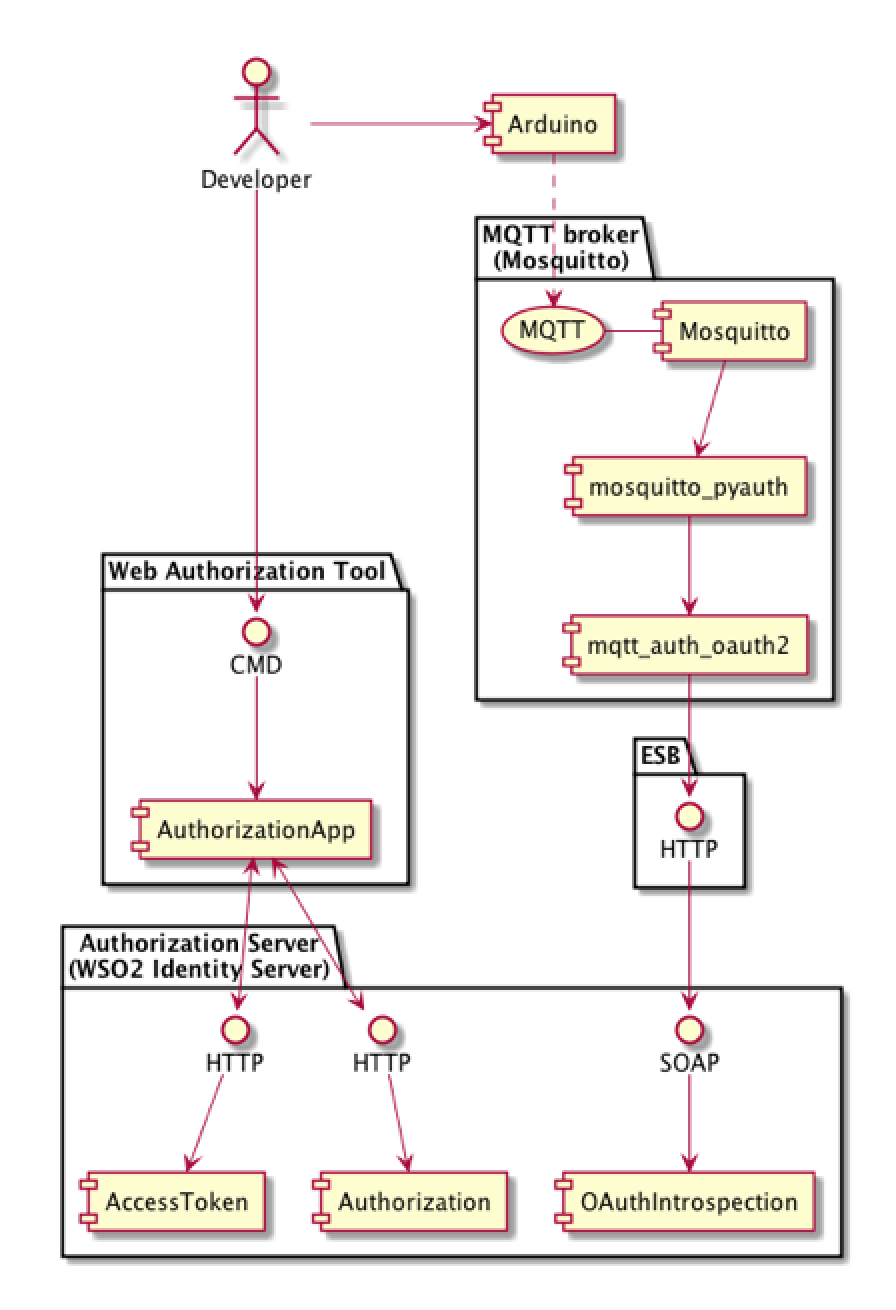
\includegraphics[width=3in]{component-diagram.png}
\caption{Component diagram of the implemented system}
\label{fig:component-diagram}
\end{figure}

\subsection{Authorization Server}
The WSO2 Identity Server~\cite{wso2-identity-server} is an open-source identity and access management
server that supports a wide variety of identity and access management protocols, including 
OAuth 2.0 and OpenID Connect amongst many others. The server offers an easy-to-use web-based console
which allows administrators to provision users, configure OAuth applications and other tasks 
that were needed as part of this exploration. 

We did not need to modify or extend the WSO2 Identity 
Server to implement the ``Authorization Server'' role defined in our architecture. However, the WSO2 Identity Server implements its own SOAP-based API for querying the validity and scopes of a token. This was not ideal to call from the message broker, and we preferred the using of the OAuth Token Introspection~\cite{richer2013oauth} API, which is a simpler RESTful API. We therefore created~\cite{oauth-introspection-blog} a simple bridge between the two APIs using the WSO2 ESB~\cite{wso2-esb}, which meant that we could swap the WSO2 Identity Server out for any other OAuth2 server that implements this API. More generally, this extension means any system that use the Introspection API can now interact with the WSO2 Identity Server.

In order to capture authorization scopes that a token is given access to, we created a JSON~\cite{json} encoding. The following example shows a scope that encodes a client who can 
write to any subtree of \emph{/topic/paul} and read/write to \emph{/scratch}:
\begin{verbatim}
[   {rw:"w", topic:"/topic/paul/#"},   {rw:"rw", topic:"/scratch"} ]
\end{verbatim}
This model uses the same syntax for wildcards as the MQTT specification, which is the logical 
and most effective approach. Because the scope list in OAuth2 is space-delimited, we could not use this JSON as-is to form the authorization scopes. To solve this, we used Base64-encoding to create simple strings that could be used as scopes. There are other solutions we could have taken, but this was expedient as it made parsing the scopes simple for the broker.

\subsection{Web Authorization Tool (WAT)}
We need to be able 
to instantiate the bearer and refresh tokens and associate the correct access control scopes with these tokens. 

This process is described in greater detail in the OAuth 2.0 
specification. In the OAuth terms, the MQTT device is the ``client''. However, we are actually
separating this into two parts: the bootstrap process, and the runtime process. The bootstrap process is a set of Web-based flows. Once this
process is complete, we then take the bearer and refresh tokens and embed these into our device, which then uses them at runtime.
In order to support these Web-based flows, we ideally needed to create a Web-application, because
part of the flow is a redirect back to that application, which needs to be Web addressable. 

However, we felt a command-line tool would be simpler and more appropriate.
To solve this, we created a command-line tool in Python that ran a simple embedded Web-application. 
This command-line tool spawns a browser with the correct URL to request a token. This is important because the user must authenticate to the Authorization server, which
then redirects that browser back to the local embedded Web server. The result is that there is no 
need to run a dedicated Web server and the command-line tool can be used to create tokens.
This tool generates a textual version of the token, suitable for cutting and pasting into other systems;
and  generates C code for the Arduino, which can be cut and pasted into the Arduino tooling to update the Arduino.
In a real environment as opposed to this prototype, we would have extended the tool to write this directly into the flash of a connected device.

In addition, we wanted to demonstrate the other end of the flow -- a non-device-based application gaining 
access to the data published by the IoT device. Of course, this application must be 
authorized by the owner of the data (the Resource Owner) to be able to access this data. Ideally this
would have been a proper Web application. However, we felt that this angle was the closest to the existing 
OAuth2 usage and so few insights would be gained from building this, so we emulated
this using the default command-line clients provided by Mosquitto. We call this aspect the Message Viewer.

\subsection{The Device}
To create our sample IoT device, we utilized an 8-bit Arduino open hardware device~\cite{arduino}, together
with the Arduino Ethernet Shield, which is a daughterboard that provides Ethernet support. 
The Arduino toolkit has a library that supports the MQTT specification~\cite{pubsubclient}.
Our device utilizes a 9-axis inertial measurement unit (IMU) that provides acceleration, rotation and
compass data -- each in 3 dimensions, to track the movement of the device. Such devices, when 
attached to a person, provide significant data on the users position, activity and exercise levels. Such
data exemplifies the problem space here: users wish to share this kind of data, but only in precisely 
controlled ways, and each user may have radically different approaches and concerns about both
data sharing and privacy. 

One important point to note is that we did not implement any TLS or encryption from the device to the MQTT broker. This was because of space requirements in the Arduino device. However, we consider this issue orthogonal to the other concerns as OAuth2 and MQTT layer cleanly sits over TLS.

\subsection{MQTT Message Broker}
Mosquitto is an open-source MQTT broker written in the C language~\cite{mosquitto}. It is highly portable. Mosquitto has a well-defined model for
adding authentication/authorization plugins~\cite{mosquitto-auth} and there are several third-party
plugins but we could not find any 
example of an existing OAuth-based plugin for Mosquitto. 

In this model, the MQTT IoT device connects to the broker, and instead of passing over a username 
and password, it sends an OAuth 2.0 \emph{bearer token}. 
%\iflong
The bearer token is a specific type of 
token supported by the OAuth 2.0 specification that was designed to support very simple client 
software. Unlike the OAuth 1.0 specification, which required the client to perform signature 
operations in order to communicate, the bearer token is a token which can be stored and sent
as proof of identity. This has its own security challenges which we discuss later.
%\fi

To create our authorization plugin we utilized the mosquitto\_pyauth~\cite{mosquitto-pyauth} project. This plugin converts from the normal
C-language based model for Mosquitto plugins into the Python language, allowing us to write the OAuth
plugin for Mosquitto in Python instead of C. 
\iflong
We did not assess the performance differences between writing in the native C model versus writing 
in Python as we were primarily aiming at experimenting with the model and the performance was adequate
for our tests. However, it would not be challenging to rewrite the plugin in pure C as most of the 
work is done by the remote Authorization Server. 
\fi

Utilizing mosquitto\_pyauth as a bridge into Python, we then wrote a Python-based plugin --
\emph{mosq-auth-oauth2} -- that validates the OAuth2 bearer token which the client passes over. 
The plugin sends this OAuth token to the \emph{OAuth Introspection Service}, 
that validates the token and returns a set of 
authorized scopes for this token. The authentication/authorization plugin then validates if 
the requested action (reading or writing to a topic) is valid against this scope.


A picture of the implemented architecture is shown in Figure \ref{fig:arduino-device} in Appendix \ref{app:ard}, where the prototype device is connected to a Mosquitto broker running on Raspberry Pi hardware.  Additionally, Appendix \ref{app:int} contains two sequence diagrams showing the system interactions: Figure \ref{fig:bootstrap-sequence-diagram} shows the sequence diagram of interactions during the bootstrap
phase, and Figure \ref{fig:runtime-sequence-diagram} shows the sequence diagram of the interactions during 
the use of the device and the Message Viewer.

\iflong
\subsection{Minor implementation issues} 
During the implementation we came across a number of issues that we considered could be improved 
in a future implementation. We did not feel that any of these could not be overcome or 
circumvented, but we did believe that they are worth documenting in order to capture the lessons learnt.
\begin{itemize}
\item Because of the nature of the authentication plugin interface to Mosquitto, it was not simple 
to use the password parameter to pass the token. Therefore we passed it as the username. 
This is an implementation specific issue, and doesn't affect the overall model. However, we would recommend creating a standard
way of passing the token over, and we would recommend this be the password field and not the userid field that was used in this experiment.
\item We did not attempt to cache the authorization decisions, or the results of the OAuth introspection.
This would be a nice enhancement that would reduce the network traffic and significantly enhance performance. 
The fact that the OAuth token has a expiry time gives an effective caching model.
\item We did not implement any model where the broker disconnects the client when the token expires, which 
would be a good extension.
\item The Base-64 encoded scopes were not humanly-readable. This meant it was harder for the user to validate the meaning of the scope request. However, in a real 
consumer facing system, we would expect the scopes to be human-readable names with proper descriptions which would be mapped by the broker into the topic hierarchy.
\end{itemize}
\fi

\section{Results}\label{sect:results}
Overall the system worked as intended, and showed the following aspects:
\begin{itemize}
\item Both IoT and non-IoT clients were able to use OAuth tokens to authenticate to the broker.
\item The broker was able to connect using a RESTful interface to the OAuth Authorization Server 
to validate tokens.
\item The broker was able to introspect the token via the RESTful interface on the Authorization Server
to retrieve a list of appropriate scopes.
\item The broker was able to use the scopes to decide on whether to authorize a publish or 
subscribe operation.
\item The Web Authorization Tool was able to implement the OAuth 2.0 bootstrap process to create Access
Tokens, which were then embedded into the MQTT clients.
\end{itemize}
However, we did find several issues during implementation, which we will discuss next.

\subsection{Refreshing the Token}
Firstly, the use of HTTP as a protocol to implement the Refresh Token flow is not ideal. 
It requires the device (in our case the Arduino client) to implement two protocols (MQTT and HTTP), which is 
inconvenient. To give an example, our IMU and MQTT code took up 97\% of the program space of the 8-bit 
Arduino on which we prototyped. The extra code for OAuth2 took us to 99\%.
Adding HTTP code for the refresh flow would have pushed us over the limit.

A fundamental issue is that the Refresh Token flow requires the device to 
produce the Client ID and Client Secret. This is a well known issue in the mobile space, and 
highlights a challenge in using the OAuth specification outside the Web application space.
This is a limitation in the design of OAuth, which is effectively based around the concept 
of a Web Application. In the Web Application model, there is a single place where the Web Application
is deployed and managed\footnote{Of course a Web Application may be deployed in multiple datacenters
for scalability and disaster recovery, but this is still logically a single place}.

In an IoT (or for example the case of a mobile phone application), the client application is deployed in 
thousands or potentially millions of places. The task of securing the Client Secret is therefore 
much harder. Microcontrollers such as the Atmel Mega used in the Arduino do
allow the code to be locked onto a device, but in any situation where the hardware is 
accessible, it is always possible for a determined hacker to break such security. This really 
depends on the value associated with compromising the security: if the reward is high enough, 
a determined hacker can utilize a Scanning Electron Microscope~\cite{silicon-investigations}.
The alternative is to issue Access Tokens with very long expiry times, where the expiry time 
is expected to be longer than the lifetime of the device, or where there is an option to update
the device with new firmware. This may be possible, but it goes against best practice for OAuth2.

A key question that arises is whether each device is considered in the OAuth2 world to be a separate Client or 
that the overall set of devices is considered to be a single Client. If each device is a unique client, then it is  to 
code the Client ID and Client Secret into each device. If a single device is compromised, it only 
compromises that devices' secrets, and they can be revoked. However, it is (as-yet) untested whether OAuth implementations
could cope with that many Clients (e.g. millions). In typical Web scenarios there are few Clients (say hundreds or maybe thousands at most).

It seems to us that it is closer to the current model to treat the set of similar devices as \textit{a Client}. In the Web world, a single 
website acts as a Client and there are thousands or millions of users, each with a token. The analogy in the IoT world
would be a single system with thousands or millions of devices attached. In this model, it would be a serious
breach of security to embed the ``global'' Client ID and Client Secret into each device, as compromising one device
would potentially compromise all of them. 

To investigate this further, we built a second phase to the experiment, where we mapped the refresh flow into MQTT.
Effectively, we created a second MQTT broker -- the Authorization Broker (AB) -- whose only job is to act as a proxy to the Authorization Server, and we used MQTT instead of HTTP to communicate from the device to this broker. 
\iflong
To explain this, let us name the two brokers: the first (existing) broker is the Data Broker (DB), where data is published and received.
The second broker is the Authorization Broker (AB).
The flow works as follows:
\begin{itemize}
\item The device attempts to connect to the Data Broker. 
\item The bearer token has expired and the connection is refused.
\item The device connects instead to the Authorization Broker (with no credentials)
\item The device passes the bearer key to the Authorization Broker
\item The Authorization Broker (or an agent attached to it) adds the Client ID and
 Client Secret and calls the real Authorization Server to refresh the token.
\item The Authorization Broker then returns the new Bearer Token to the client.
\item Finally the client disconnects from the AB and tries again to connect to the DB with the new Bearer Token.
\end{itemize}

\fi
During the implementation we discovered some interesting sub-issues specific to this refresh flow.
Firstly, it is not trivial to send a message to a single device using MQTT. As the system is a pure pub/sub network
there is no built-in way of targeting a single device. Obviously we did not desire to broadcast the refresh token to 
all devices as that could be misused. To solve this, we implemented a special authentication rule and topic hierarchy on the AB that allowed us to securely send a message just to a single client.

Secondly, the OAuth specification optionally allows the Authorization Server to refresh the Refresh Token as well. 
This is a significant issue in a device-oriented world, because the HTTP call to the Authorization Server is unreliable.
If the device ends up ``out-of-sync'' with the Authorization Server, then the device will need to be re-registered.  In the Web world, this is easily sorted and happens
frequently - it is just a case of the user re-authorizing. 
With devices, this may not be possible as there is often no Web Browser and UI -- which is required in this case.
To get round this, we worked with the WSO2 Identity Server development team
to add an option to allow us to keep the refresh token constant. We would recommend any OAuth2 server that is being used for IoT devices would avoid changing the 
Refresh Token with every refresh. This applies to IoT devices using HTTP as well as MQTT or other protocols. Another option would be to use a reliable protocol to transmit the updated refresh token end-to-end from the Authorization Server to the device.

Another concern is whether this model (where any device can connect to the authorization broker and pass over a Refresh Token) is a security
hole. Certainly we could protect it in some regard, but this may not improve matters. If we use a unique credential per device, we have created a circular issue (i.e. how do we manage that credential?). 
If we use a default credential that is the same for all devices, an attacker needs only to break one device to break this.
On the other hand, without a refresh token, the attacker cannot do any real harm. They can cause denial-of-service by issuing 
many requests, but this could be prevented by standard DoS firewall techniques. On the whole, we felt this model was better than 
having a unique Client ID/Client Secret per device or having the same Client ID/Client Secret on all devices.

\subsection{Changing the scope}
The third issue that was identified during our work was that of updating the scope.
In many cases, one might want to change the permissions associated with a device after the firmware
has been loaded. In many Web systems, to change the scope of a token is done by re-issuing the token. As we have discussed, this is not appropriate for many embedded devices or those without a UI and browser. 
%There are two approaches to solve this.
%Firstly, one can refresh the firmware. However, this is difficult in many cases. Especially with
%small devices the programming may require special hardware. If \emph{over-the-air} re-programming 
%is allowed then that can also enable security concerns such as malicious re-programming. 
%Many devices have the code locked to prevent it being updated or read.

A better approach is to update the scope of the existing token. This would remove the burden 
from the device and deal with it purely at the Authorization Server. However, as
currently specified, the OAuth 2.0 specification has no explicit mechanism to allow this. That said, 
the specification does not prevent it either, but it would need to be an implementation specific 
approach and therefore would not be interoperable. We see this as an area where the 
challenges of the IoT should influence the development of OAuth or other similar 
protocols, as well as the capabilities of OAuth implementations.

\section{Conclusions and Further Work}\label{sect:conc}
In this paper, we have shown that a standardized federated, dynamic, user-directed authentication and authorization model
can be adapted from the Web for use in IoT devices. We have argued that this model
is important for the concept of privacy with respect to IoT devices and the data that they 
generate and use. We have identified a number of issues, including both minor implementation issues as 
well as more fundamental issues where we propose further research. This was 
the first such implementation of OAuth2 with MQTT.

As a result of this work, there are several recommendations that we propose.  These include the need for clear standardization of where to put the token as well as limiting the OAuth2 token size to some reasonable limit - at least for IoT use. Also there is a need to define a clear MQTT flow for refresh and avoid refreshing the refresh token. Finally, there is some concern over the AB's security and the need to be able to modify scopes.  Two of these findings apply also to the use of OAuth2 with any protocol, including HTTP, when used with IoT devices: the need for the refresh token to be constant (or transmitted reliably), and the need to allow scopes to be modified for existing tokens. 

While there were some issues with implementing FIAM for IoT using OAuth2 with MQTT, the benefits of building on existing widely implemented and deployed protocols are significant. Many years of work and review have gone into the security of OAuth2, and from this work we can state that it is possible to re-use this work with IoT devices and new protocols.

Several areas for further research emerge from this work. A formal model and proof of security attributes for the use of OAuth2 with MQTT and in particular, the refresh flow, would be beneficial. Similarly, it would be valuable to analyse the performance of this model and understand the extra cost of using OAuth2 compared with traditional security. One aspect we did not consider was allowing more than one OAuth2 Authorization Server to be used with a single broker, which would merit research.

We wish also to investigate the use of OAuth2 with CoAP and other protocols for IoT. During discussions of this work with device implementers, a common request has been to create an Arduino ``shield'' that embodies the MQTT, OAuth2 and TLS behaviour completely, which would make an interesting project.
Finally, we believe that some investigation is merited into whether the OpenID Connect specification could add any benefits over OAuth2 in the IoT space.

% use section* for acknowledgement

% trigger a \newpage just before the given reference
% number - used to balance the columns on the last page
% adjust value as needed - may need to be readjusted if
% the document is modified later
%\IEEEtriggeratref{8}
% The "triggered" command can be changed if desired:
%\IEEEtriggercmd{\enlargethispage{-5in}}

% references section

% can use a bibliography generated by BibTeX as a .bbl file
% BibTeX documentation can be easily obtained at:
% http://www.ctan.org/tex-archive/biblio/bibtex/contrib/doc/
% The IEEEtran BibTeX style support page is at:
% http://www.michaelshell.org/tex/ieeetran/bibtex/
%\bibliographystyle{IEEEtran}
% argument is your BibTeX string definitions and bibliography database(s)
\bibliographystyle{splncs03}
\bibliography{references}

\appendix
\FloatBarrier
\section{Picture of the Implemented Prototype}\label{app:ard}
\begin{figure}[!t]
\centering
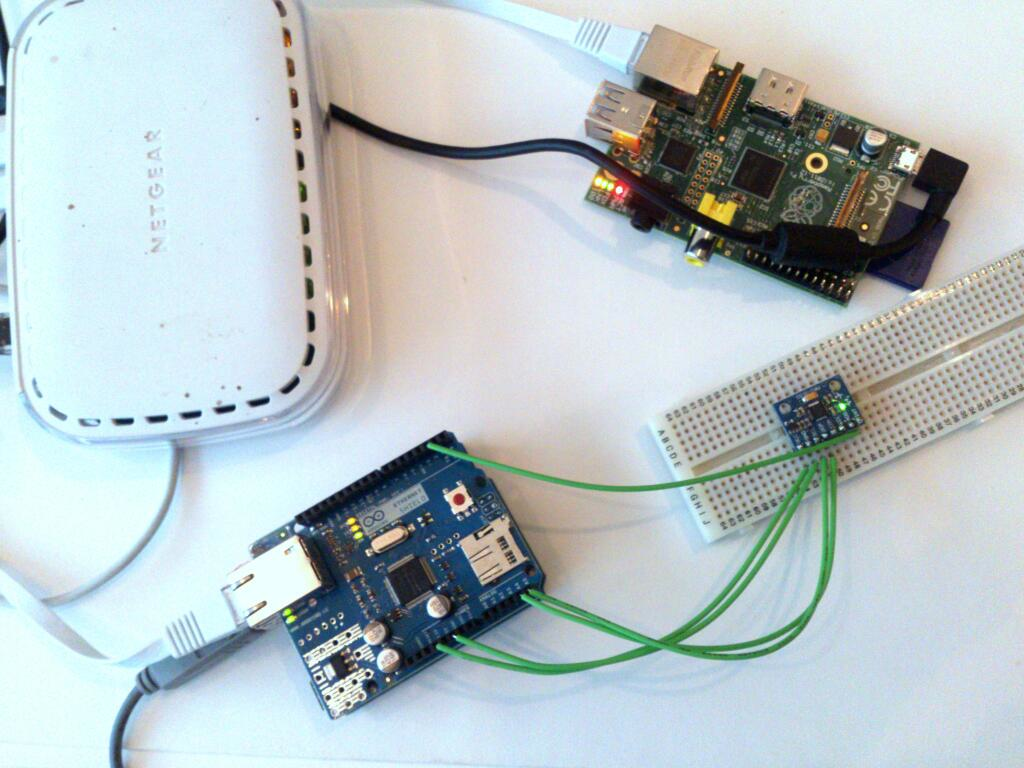
\includegraphics[width=4in]{arduino-device.png}
\caption{Arduino Device prototype with 9-axis IMU}
\label{fig:arduino-device}
\end{figure}
\FloatBarrier
\section{Interaction flows}\label{app:int}
\begin{figure}[!t]
\centering
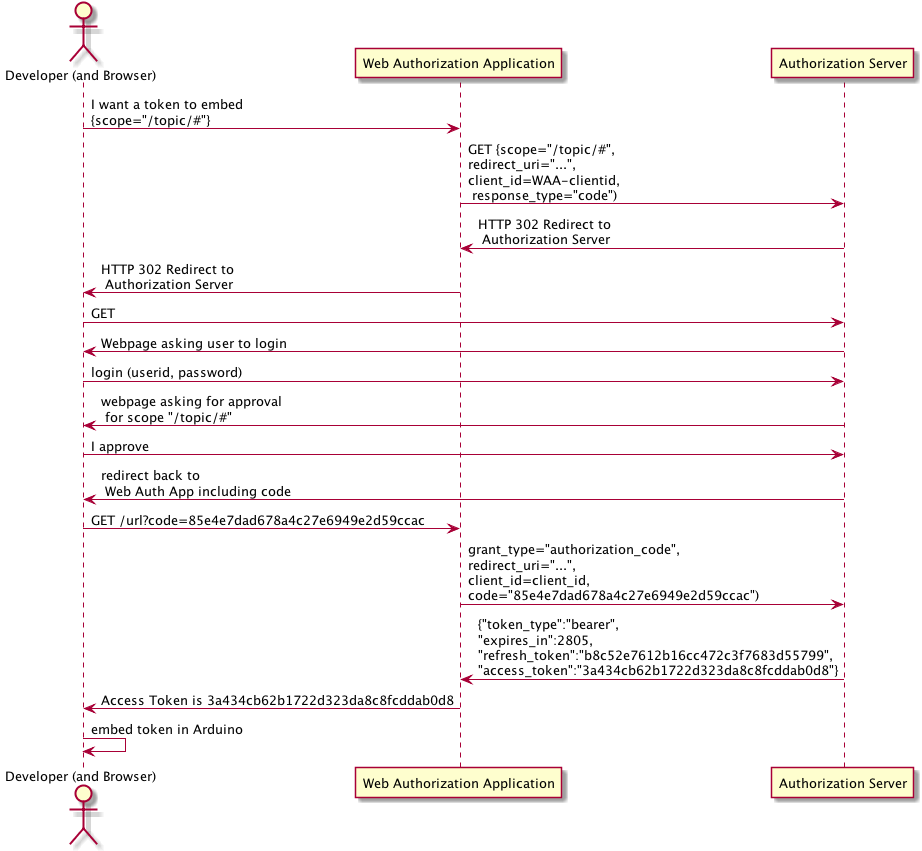
\includegraphics[width=3in]{bootstrap-sequence.png}
\caption{UML Sequence Diagram demonstrating the bootstrap phase}
\label{fig:bootstrap-sequence-diagram}
\end{figure}
\FloatBarrier
\begin{figure}[!t]
\centering
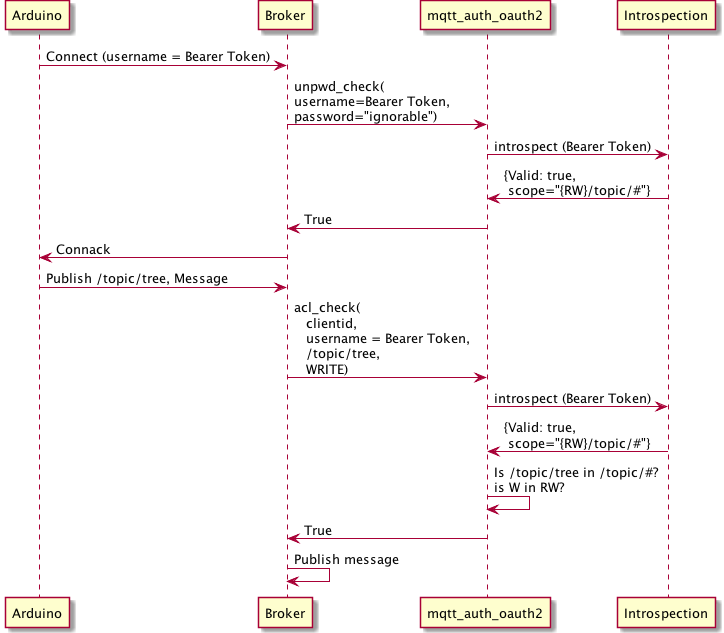
\includegraphics[width=3in]{runtime-sequence.png}
\caption{UML Sequence Diagram demonstrating OAuth access control check}
\label{fig:runtime-sequence-diagram}
\end{figure}
\FloatBarrier
\section*{Acknowledgments}
Thanks to the Mosquitto project and Eclipse Paho projects for the excellent code, to Prabath Sidiwardena for help with OAuth2 and the WSO2 Identity Server. Finally, thanks to Jane for proof-reading.




% that's all folks
\end{document}


